%From introduction to be added here

%Data transfer and storage are expensive for research data centers as well as Internet-of-Things (IoT) devices\footnote{Dataversity, \href{https://www.dataversity.net/internet-things-vs-edge-computing-processing-real-time-data/}{Internet of Things vs. Edge Computing: Processing Real-Time Data}, accessed online 12/2018}.

%(including inter/multidisciplinary, intersectoral and, where appropriate, gender aspects)

\subsubsection{Introduction, objectives and overview of the research program}
\label{sec:introRO}

%\noindent{\color{blue}{State of the art and how \acronym will go beyond it}.}
%brief description, international bibliographic references, cite the consortium

High Energy Physics studies the basic constituents of matter and searches for possible extensions of the theory describing them, called the Standard Model. 
One of the main experimental tools available for this study is the LHC. 
At the LHC, particle beams are accelerated to high energies and collided every 25 ns.
The products of the collisions, called \textit{events}, are analyzed by scientists operating four main particle detectors: ALICE, ATLAS, CMS and LHCb\footnote{CERN, \href{http://cds.cern.ch/record/1997374}{The LHC Experiments}, CERN Document Server}.
As the LHC in Geneva collides protons 30 million times per second and recording them all would be prohibitive for the current data acquisition and storage systemsm 
each experiment has a \textit{trigger system} composed of hardware and software.
The trigger system analyzes those events with a maximum delay of micro- to milliseconds and selects which ones to be kept for further analysis. 
As detailed in Secs.~\ref{sec:trainingcontrib} and~\ref{ss:competence_44}, researchers in the \acronym consortium are experts on the trigger systems of their respective experiments, and have been extending the physics program of their experiments using novel real-time data-taking techniques\footnote{e.g. Gligorov and Fitzpatrick, \href{http://cds.cern.ch/record/1670985}{Anatomy of an upgrade event in the upgrade era, and implications for the LHCb trigger}, CERN Document Server. ALICE Collaboration including Christiansen, \href{https://cds.cern.ch/record/2011297/files/ALICE-TDR-019.pdf}{Technical Design Report}, CDS Document Server, ADD ATLAS TRIGGER PAPER}. 
In particular, they have pioneered a technique that saves only the highest level of information, rather than the raw data as it is traditionally done. 
This means that the detector information is analyzed in real time, and only smaller, high-level quantities are recorded while the larger raw data is discarded. 
This approach allows a greater number of events to be analyzed and a much increased sensitivity for measurements and discoveries\footnote{CMS Collaboration including Pierini, \href{https://arxiv.org/abs/1604.08907}{Search for narrow resonances in dijet final states at $\sqrt{s}$ = 8 TeV with the novel CMS technique of data scouting}, Phys. Rev. Lett. 117, 031802 (2016). ATLAS Collaboration including Boveia, Starovoitov, Dunford and Strom, ADD HERE TLA REF, LHCb collaboration including Gligorov, Borsato ADD HERE DARK PHOTON REF}.
Following these successes within the individual experiments, \textbf{the \acronym network pools the expertise of RTA experts of all main LHC experiments to train a new generation of researchers focused on RTA techniques. Supervised by both physicists and computer scientists in \acronym, the ESRs will exploit innovative ML techniques and hybrid computing architectures to upgrade the trigger systems of LHC experiments for the next LHC data taking periods (Run-3, starting in 2021, and Run-4, starting in 2025) where the volume of data will increase even further, and perform physics analysis with these improved systems that will provide precise probes of the Standard Model.} 

\acronym's ESR projects employ RTA in research as well as in projects that are useful to industry and society. 
Time-to-insight from raw data is a crucial benchmark for a competitive and effective use of the information. For this reason, advancement in terms of fast and efficient data analysis and decision-making are required by society and the commercial sector, and a selection of industrial use cases sharing common issues with HEP has been chosen as integral part of the \acronym research and exploitation program as described further in Sec.~\ref{sec:exploit}.  
RTA is a key point for improving transport: the information on the position of vehicles / public transport and their possible routes are transmitted to a central analysis system, so that the traffic conditions around it are analyzed and a forecast is made. All of this needs to be done on a timescale that is short enough for a city to modify its traffic light system to avoid congestion, or to reroute other vehicles to avoid delays. This requires both ML and hybrid computing architectures (GPU) for algorithm training, similarly to the solution of complex problems such as tracking particles in a HEP detector. 
The detection of a driver's behavior (e.g. drowsiness) in fleets of cars needs to happen in the timescale of milliseconds to preserve the safety of the driver, and detection of malfunctioning components in industrial processes must trigger maintenance before the component breaks. Both those use cases require the optimization of advanced algorithms on limited computational resources, much like HEP's trigger systems.
Another use case for RTA in industry is fraud detection, where a decision on whether a transaction is allowed or not needs to be made on a timescale of seconds. 
While ML algorithms trained to detect outliers are the current state of the art for this purpose, their black box approach raises interpretability and explainability challenges. 
This is one of the topics tackled by \acronym: knowledge-based approaches for the induction of explicit decision rules are useful both for increasing the accountability of fraud detection algorithms and for HEP trigger systems where every decision to discard an event is final and must be completely understood. 
\textbf{The cross-talk on RTA between academia and industry in \acronym will lead to concrete deliverables that contribute to improving European transport as per the H2020 Societal Challenge for Smart, green and integrated transport\footnote{\href{https://ec.europa.eu/programmes/horizon2020/en/h2020-section/smart-green-and-integrated-transport}{Smart, Green and Integrated Transport summary, H2020 website}, Accessed online 12/2019}, to enhance the capabilities and reproducibility of decision-making in finance and to improve industrial processes.}

%originality and stuff - add here

\subsubsection{Network goals and research objectives}

\acronym trains researchers in ML, AI and data analysis and hybrid computing architectures, in order to enable RTA for the advancement of decision-making as well as monitoring and discoveries in both research and industry. 
The network's goal defines the four main research topics for \acronym, reach corresponding to a research Work Package (WP) detailed in the following section.
Each of the research topics requires collaboration between industry and HEP, and has concrete objectives beyond the state-of-the-art that can be achieved with this network, linked to concrete deliverables. 

%\vspace{-2mm}
%\begin{multicols}{2}[]
%%\small
\begin{enumerate}%{\leftmargin=1em}

\item The first research topic concerns the use of \textbf{ML, AI and advanced data analysis} in RTA techniques.
%The sheer size of the datasets collected by scientific experiments has lead researchers in HEP to use advanced data analysis methods normally used in industry, such as ML and AI. 
ML techniques are by now ubiquitous in both HEP and industry, in order to optimally analyze raw, unstructured data. In \acronym we will further extend their use in RTA and event reconstruction, paying particular attention to their understandability and reproducibility (see research topic 4).   
Meta-analysis (benchmarking) is also necessary to understand the algorithm performance prior to using them in RTA, which often occurs in resource-constrained environments.
%and industry.
The \acronym ESRs will:
\begin{itemize}
\item design and use of a variety of ML algorithms for RTA (GAN, RNN, Deep Learning) $\rightarrow$ HEP and commercial software toolkits (ADD DELIVERABLES); 
\item implement efficient real-time object and event reconstruction $\rightarrow$ software for HEP experiment triggers (ADD DELIVERABLES);
\item benchmark and optimize RTA algorithm performance $\rightarrow$ inter-experiment, inter-sector toolkits (ADD DELIVERABLES). 
\end{itemize}

\item The second research topic focuses on the design of innovative \textbf{hybrid computing architecture} solutions in hardware/software, given that the complexity and rate of LHC data and beyond does not allow standard processors or data analysis techniques to be competitive\footnote{J.P. Vlimant, \href{https://erez.weizmann.ac.il/pls/htmldb/f?p=101:58:::NO:RP:P58_CODE,P58_FILE:5393,Y}{Machine Learning in Charged Particle Tracking}, Hammers and Nails ML\&HEP Conference, 2017}. 
As an example, 
The \acronym ESRs will:
\begin{itemize}
\item use Field Programmable Gate Arrays $\rightarrow$ trigger improvements for LHC experiments (ADD DELIVERABLES);
\item use Graphic Processing Units $\rightarrow$ significant speed-up for HEP and industrial ML and RTA techniques (ADD DELIVERABLES);%Ximantis
\item design parallelized and multithreaded algorithms $\rightarrow$ RTA software needed for the increase in LHC data and for improving financial transactions (ADD DELIVERABLES).
\end{itemize}

\item The third research topic concerns \textbf{real-time decision making in physics and industry}. 
The outcomes of the previous research topics will be applied to concrete physics cases and industrial challenges. 
As an example for the physics motivations behind \acronym, we consider the SM prediction that the weak force couplings to all lepton types are equal (Lepton Flavor Universality, or LFU), and that the overall number of leptons of a given type does not change in interactions (Lepton Flavor Violation, LFV). 
Recent measurements published by LHCb indicate that in decays of beauty mesons, LFU might be violated (see e.g. Phys. Rev. Lett. 113(2014)151601 and JHEP08(2017)055), making this one of the most interesting topics for the near-future of particle physics and one that needs RTA to be explored. 
The \acronym ESRs will: 
\begin{itemize}
\item Deploy improvements from real-time reconstruction and hybrid architectures in trigger systems $\rightarrow$ possible confirmation of hints of physics beyond the SM from LFU and precise results on heavy ion physics (ADD DELIVERABLES);
\item Extension of RTA techniques in HEP trigger systems where raw data is discarded $\rightarrow$ results that probe unexplored ground in the Higgs and Dark Matter sectors (ADD DELIVERABLES);
\item Use RTA to improve transport and safety of fleets $\rightarrow$ inputs to connected cities, extended transport apps and in-vehicle software (ADD DELIVERABLES)
\end{itemize}

\item The fourth research topic concerns efficient and accountable \textbf{monitoring} of complex processes and the preparation for physics \textbf{discoveries}. 
This has a strong motivation in HEP. 
There are many observed phenomena that are still not included in the SM (e.g. dark matter [LINK BOVEIA DOGLIONI ANN REV]). 
The leading predictive theories such as Supersymmetry have only yielded negative results, prompting researchers to look towards unexpected manifestations in the detector that would be missed using the current trigger algorithms. 
The \acronym ESRs will:
\begin{itemize}
\item Implement outlier detection techniques $\rightarrow$ not-yet-theorized discoveries at the LHC and improved fraud detection algorithms (ADD DELIVERABLES);
\item Study and design rule-induction algorithms as complement to ML to improve accountability and understandability $\rightarrow$ RTA for fraud detection and HEP triggers (ADD DELIVERABLES);
\item Implement ML techniques in RTA for IoT-ready industrial production chains $\rightarrow$ real-time forecasting for interventions (ADD DELIVERABLES);
\end{itemize}

\end{enumerate} 
%\end{multicols}
%\vspace{-2mm}
%\vskip 5mm

%The connections between the consortium expertise, the different work packages
%and the overall \acronym strategy are shown in 
%Fig.~\ref{fig:scienceStructure}. 

The research objectives defined in \acronym go beyond the present state-of-the-art. 
They can only be achieved through the constitution of a multidisciplinary team, providing the required research resources and the appropriate \textbf{training}. 
%shown in Fig.~\ref{fig:scienceStructure}
%Therefore, outstanding training will be an objective in itself.
%How the individual projects of the recruited researchers will be integrated into -- and contribute to
%-- the overall research program is described in more detail together with the research methodology in Sec.~\ref{sec:metho}.  
The concrete outcomes of \acronym will be \textbf{whitepapers, peer-reviewed publications and software toolkits} for the research objectives, that would not be possible without the expertise in this network. 
We also believe that the experience gained with \acronym will lead to new interdisciplinary training models for scientists in other data-intensive domains.
With four in ten companies reporting a shortage of analytical skills\footnote{\href{http://www.forbes.com/sites/gilpress/2015/04/30/the-supply-and-demand-of-data-scientists-what-the-surveys-say/}{Supply and demand of data scientists}, Forbes 2015}, we believe that the proposed training program will increase the growth and competitiveness of European research, both in the academic and industrial sectors, while placing the foundations for a balanced career development model.

\subsubsection{Research methodology and approach}

ADD WPs AND FIGURE HERE 

Add the steps that I removed from the figure. Maybe too vague though.  

%one-paragraph summary of each of the WPs (10-12 lines)
%include how this will be explored (credibility/feasibility here)
%highlight inter/multidisciplinary 
%Explain how the individual ESRs fit into the WP in table 
%use a figure to illustrate relationship?

%TODO: shorten this to one sentence, remove the blue
\subsubsection{Originality and innovative aspects of the research program} 
\label{sub:Originality}
%Expand on the state of the art: why is this original, innovative ad timely
%Refer to the state of the art in the first paragraph

Add gender!! We got the benchmark of 40\% with node responsibles

\noindent {\color{blue}{1. Researchers from \acronym learn to process large datasets using novel analysis techniques}.}
%  \begin{wrapfigure}{r}{0.7\textwidth}
%%\begin{figure}{l}{\textwidth}
	%\vspace{12mm}
%	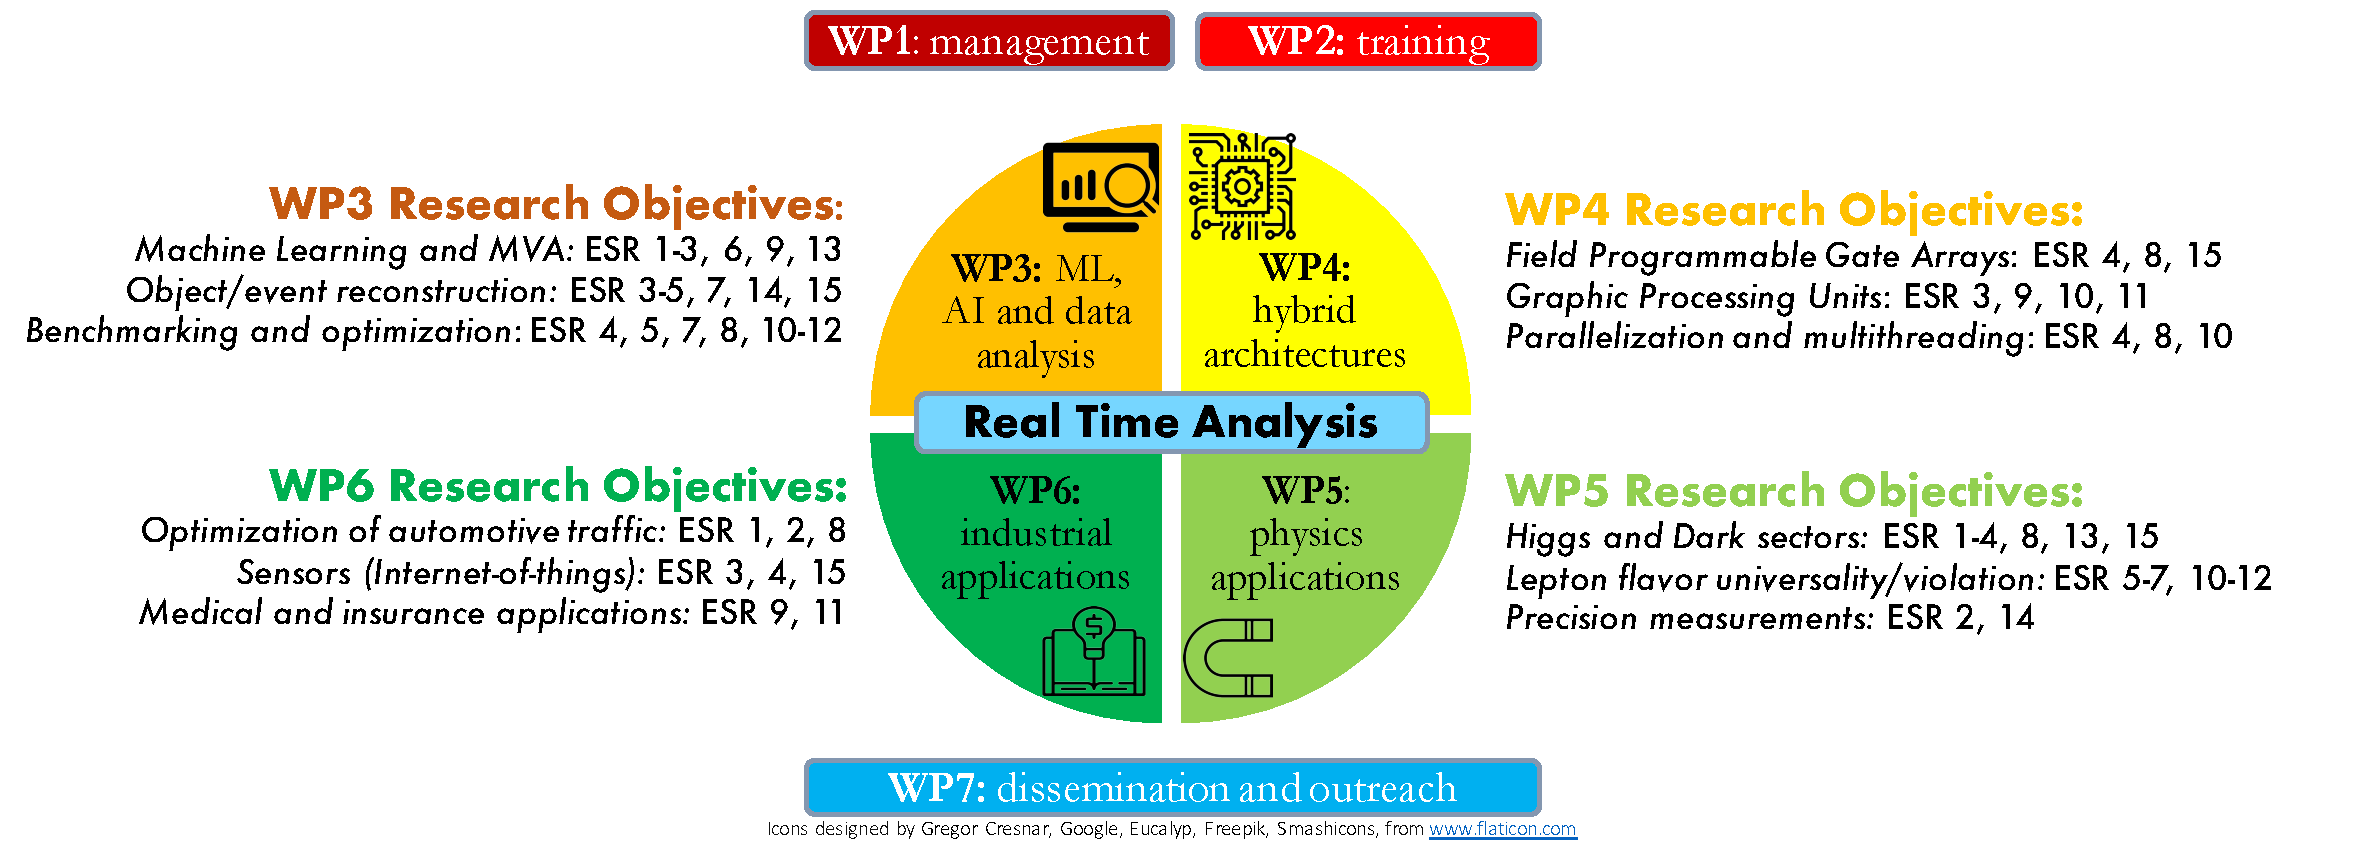
\includegraphics[width=0.7\textwidth]{figs/WPs} %scienceStructure_2.pdf}
%    \vspace{-5mm} 
%	\caption*{Figure 2 : Structure and Research Objectives of the Work Packages.\label{fig:WPs}}
     %\vspace{-5mm} 
%%\begin{figure}	
%\end{wrapfigure}
A large part of the novelty of this proposal is the volume of data which will be processed, comparable to the largest commercial tasks. 
% MLD this is a great sentence but it is just out of place here
%This is true across both academic and non-academic applications:
%an estimated 90$\%$ of generated data is considered too expensive to store\footnote{\href{http://www.mckinsey.com/insights/business_technology/big_data_the_next_frontier_for_innovation}{2010 report on Big Data by McKinsey\&Company.}}.
One can compare Facebook and e.g. the LHCb collaboration.
%MLD I switched to numbers because then the comparison is more powerful (also shorter!)
The former processes $O(100)$ petabytes of data per year and spends 500M dollars a year on computing\footnote{Facebook, \href{http://www.datacenterknowledge.com/the-facebook-data-center-faq-page-three/}{The Facebook Data Center FAQ}, 2010.} while the latter processes  $O(1000)$ petabytes of data per year and spends around 7M dollars a year on computing\footnote{Private communication, \href{mailto:peter.clarke@ed.ac.uk}{Prof. Peter Clarke}, University of Edinburgh.}.
The essential difference is that Facebook stores and distributes this data to its users while LHC experiments largely process and then dispose of the data.
%MLD I felt this was not needed to make the above argument. It removes your figure 3 but see my comment from the email. 
%An example of this are the physics searches and measurements performed solely using trigger information.
%In these searches only a small fraction of each event, regardless of whether LHC experiments are able to record it for offline reconstruction or not, is saved for further processing. 
%This overcomes the storage limitations and allows to be more than an order of magnitude more sensitive to certain new particles (e.g. associated to Dark Matter, as in Fig.3).

To achieve and go beyond this, the LHC experiments need a more systematic application of RTA, machine learning and hybrid architectures for HEP. Examples are methods using Deep Learning techniques, which build high-level features from raw data (ESR1 and ESR2), using Recurrent Neural Networks (RNNs), which learn ordered patterns in the data and can be applicable both to tracking and to model paths taken by vehicles (ESR10), and Generative Adversarial Networks (GAN) for anomaly detection techniques (ESR13).
This paradigm shift can be used in industry as well, while the research environment can benefit from a generation of ESRs trained in industrial grade algorithms and tools. 

%\begin{wrapfigure}{r}{0.4\textwidth}
%	\vspace{-4mm}
%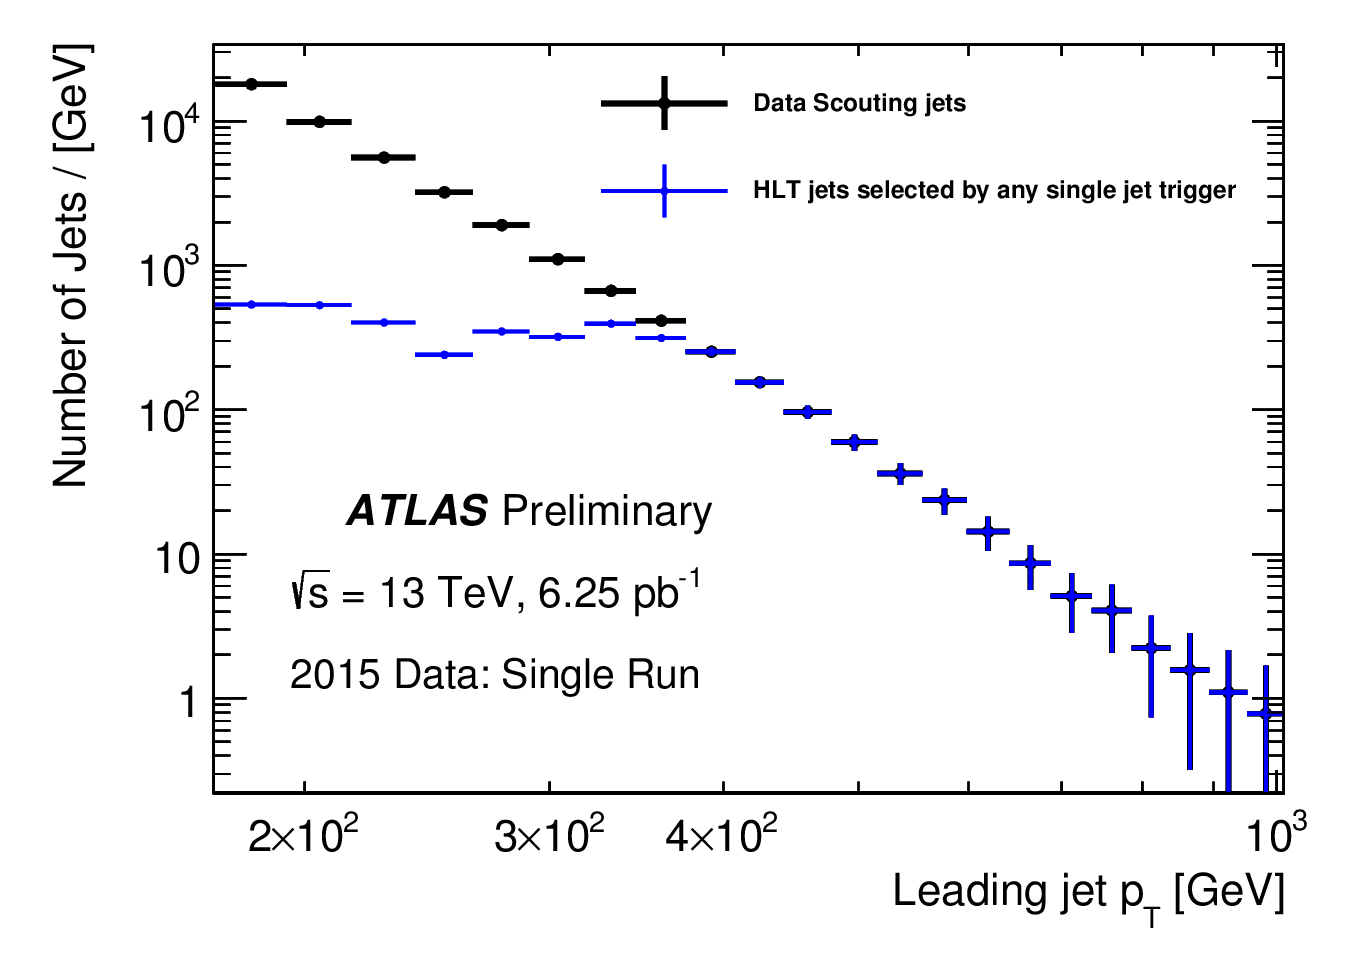
\includegraphics[width=0.4\textwidth]{figs/TLA.png} 
%    \vspace{-10mm} 
%    \caption*{Figure 3: Example of the number of events using traditional techniques (blue) compared to a trigger-level analysis (black)
%in the search for new particles. Main analyzers: Boveia, Doglioni, Starovoitov, Dunford. \label{fig:TLA}}
%\vspace{-4mm}
%    \end{wrapfigure}
%    \vspace{-3mm} 
%Real-time analysis, machine learning and hybrid architectures have so far not been systematically
%applied to HEP problems. 
%Moreover, even where toolkits exist for HEP,
%notably \tmva\ or \scikit\, they are little more than a collection
%of individual algorithms applied in an ad-hoc manner.
%The research program of \acronym is developed coherently around 
%four main research questions that are at the forefront of 
%the long-term goals of all major LHC experiments. 
%which work against each other, 
%one generating examples and the other classifying them. 
%The classifying network gets a normal score, while 
%the generating network is scored when it can create an example	
%that escapes the classifier, so to make the classifier more 
%sensitive to non-standard cases as it is essential in RTA
%where rare, non-standard but interesting events risk being lost for good. 

%%CD: possible text about machine learning
%An additional driving challenge for the \acronym research program is the continuous need for improvement of background rejection
%techniques once the data has been taken. The discovery of the Higgs boson in 2012, which lead to the award of a Nobel Prize in Physics, has 
%opened the door to a whole new set of measurements of the properties of this new particle and possible discoveries 
%of deviations from the Standard Model. However, the frequency with which
%the Higgs boson particle is produced is minuscule compared to the rates of the backgrounds yielding the same detector signatures as the Higgs boson.  
%An efficient background rejection is key for both measurements involving the Higgs boson and similarly rare particles. 
%The need for novel techniques that only select the interesting events and reject the background is acute, in high energy physics and in
%commercial applications alike. The first challenge of analyzing events in real-time addressed by \acronym also has similar needs: 
%the current paradigm of triggering on simple features 
%ignores the growing importance of the analysis of raw, unstructured, data across both academia
%and industry. For both issues, a series of techniques known as machine learning, multivariate analysis, and 

\noindent {\color{blue}{2. The \acronym program of searches and measurement could lead to breakthroughs in our understanding of nature}}
Research topics chosen to drive conceptual developments within \acronym have potential to lead to the discovery of new physics beyond the Standard Model, but only RTA techniques enable full exploitation of the LHC dataset. 
%the full statistical reach of the LHC data to be exploited. 
%Only RTA techniques will enable such discoveries. 
ESRs working on physics topics will target common challenges, e.g. when real-time algorithms and reconstruction techniques are not sufficiently advanced to distinguish signal from noise, or when the statistical power of the dataset is not fully exploited if objects are reconstructed with traditional techniques. 
%The advanced tools under design in \acronym
%will allow the real-time systems of LHC 
%experiments to improve coherently. 

% MLD this sudden detailed motivation of the physics seems out of place. This section is supposed to be motivating why the training program is unique. Also the level of detail here is not consistent with other parts. 
Examples include studies of lepton flavor and its conservation and universality in different final states and experiments (ESR 5-7, 9, 11-12), and dark matter mediators and new light particles\footnote{M. Chala et al, \href{http://arxiv.org/abs/1503.05916}{Constraining Dark Sectors with Monojets and Dijets}, JHEP 1507 (2015) 089.}.
The volume of data needed to be sensitive to these rare processes is the perfect testing ground for improved real-time techniques for ESR1 and 8.  
RTAs looking for dark matter mediators in ESR13 and 15, and the search for new particles of ESR3 and 4 using ML have never been performed at the LHC, nor have generic searches for rare new phenomena as in ESR2.
Measurements in ESR2 and 15 precisely probe the SM in the Higgs and heavy ions sectors. 

The choice of physics topics that all need RTA to achieve beyond-state-of-the-art results ensures advancement in detector development and contribution to major advances in key analyses of LHC data.
%paving the way to understand the main questions of our universe. 

\noindent {\color{blue}{3. ESRs in \acronym deploy and disseminate their research at a unique time for particle physics}.}
As highlighted by the HEP Software Foundation Whitepaper$^{4}$, the period 2019-2023 is ideal for this R\&D in HEP, as it is a time of transition between LHC data taking periods that will be necessary to prepare for an upgrade of the LHC accelerator where the amount of data delivered will make RTA techniques  the key to pursue the physics programs of the four main LHC experiments.
The systematic optimization of HEP experiments by \acronym will boost the performance of the current and planned upgrades of the CERN based accelerator experiments.
Furthermore, the developed toolkits will be advertised at international conferences and thus the developed methods will shape the online event selection of all future HEP experiments. 

\noindent {\color{blue}{4. \acronym researchers develop techniques and infrastructures that can be exploited in industrial applications, as well as in HEP}.}
The close links of the research institutes of the consortium with the industry partners means that the ESRs will directly drive the development of novel industrial products, while also bringing professional methods of data mining that are exercised in large companies into the academic environment. 
Most modern methods applied in research can in this way be transferred more easily to industry applications in automotive traffic optimization (ESR1-2, 6, 8) and analysis of sensor data for IoT and medical applications (ESR3-4, 9, 11, 13, 15).
%JA: not , 14 (??)) 
The proposed algorithms and the use of ML methods on these scales of data are novel to both HEP and industry. 
By exposing industry-grade methods to the volume and complexity of HEP data, we will stimulate their development in a complementary way for the benefit of industry.


